\documentclass{beamer}
\usepackage[utf8]{inputenc}
\usepackage{xeCJK} 
\usepackage[T1]{fontenc}
\usepackage{mathabx}
\usepackage{amsmath} 
\usepackage{mathpazo}
\usepackage{bibentry}

\usetheme{Boadilla}
\usecolortheme{wolverine}
\useoutertheme{miniframes}

\title{VP160 Recitation Class II}
\subtitle{Kinematics}
\author{Zeyi Ren}
\institute{UM-SJTU Joint Institute}

\begin{document}

\maketitle

\frame{\tableofcontents}

\section{Cartesian Coordinates}
\begin{frame}{Kinematics in 3D: Cartesian Coordinates}
  By convention, we write$$
  \frac{d\alpha}{dt}=\dot{\alpha},\quad \frac{d^2\alpha}{dt^2}=\ddot{\alpha}$$for convenience.\pause
  \begin{block}{Basic formulas in Cartesian Coordinates}
  $$ 
  \vec{r} = x\hat{n_x} + y\hat{n_y} + z\hat{n_z}$$
  $$
  \vec{v} = \dot{x}\hat{n_x} + \dot{y}\hat{n_y} + \dot{z}\hat{n_z}$$
  $$
  \vec{a} = \ddot{x}\hat{n_x} + \ddot{y}\hat{n_y} + \ddot{z}\hat{n_z}
  $$
\end{block}
\end{frame}

\section{Cylindrical and Spherical Coordinates}
\begin{frame}{Kinematics in 3D: Cylindrical Coordinates}
  \begin{block}{Basic Formulas in Cylindrical Coordinates}
    \begin{align*}\vec{r}&=\rho\hat{n_\rho}+z\hat{n_z}\\
  \vec{v}&=\dot{\rho}\hat{n_\rho}+\rho\dot{\phi}\hat{n_\phi}+\dot{z}\hat{n_z}\\
  \vec{a}&=(\ddot{\rho}-\rho\dot{\phi}^2)\hat{n_\rho}+(\rho\ddot{\phi}+2\dot{\rho}\dot{\phi})\hat{n_\phi}+\ddot{z}\hat{n_z}
  \end{align*}
  % $$\vec{r}=\rho\hat{n_\rho}+z\hat{n_z}$$
  %   $$\vec{v}=\dot{\rho}\hat{n_\rho}+\rho\dot{\phi}\hat{n_\phi}+\dot{z}\hat{n_z}$$
  %   $$\vec{a}=(\ddot{\rho}-\rho\dot{\phi}^2)\hat{n_\rho}+(\rho\ddot{\phi}+2\dot{\rho}\dot{\phi})\hat{n_\phi}+\ddot{z}\hat{n_z}
  %   $$
\end{block}\pause
  \textcolor{blue}{Tips:}\\
  \begin{itemize}
    \item if $z=0$, they become kinematics formulas in polar coordinates(see next slide).\pause
    \item Very useful, do remember this set of formulas, otherwise you may have to
    derive them by yourselves during the exam!
  \end{itemize}
\end{frame}

\section{Polar Coordinates}
\begin{frame}{Kinematics in 2D: Polar Coordinates}
  \begin{block}{Basic Formulas in Polar Coordinates}
    \begin{align}\vec{r}&=r\hat{n_r}\\
      \vec{v}&=\dot{r}\hat{n_r}+r\dot{\theta}\hat{n_\theta}\\
      \vec{a}&=(\ddot{r}-r\dot{\theta}^2)\hat{n_r}+(r\ddot{\theta}+2\dot{r}\dot{\theta})\hat{n_\theta}
      \end{align}
  Can be seen as a special case of cylindrical coordinates when $z=0$.
  \end{block}\pause
  \begin{block}{Relations with cartesian coordinates}
    $$x=rcos\theta,\ y=rsin\theta$$
    $$d\vec{r}=dr\hat{n_r}+rd\theta\hat{n_\theta},\ |d\vec{r}|=\sqrt{(dr)^2+(rd\theta)^2}$$
  \end{block}
\end{frame}

\begin{frame}
  \textcolor{blue}{Examples}
  \begin{figure}[htbp]
  \centering
  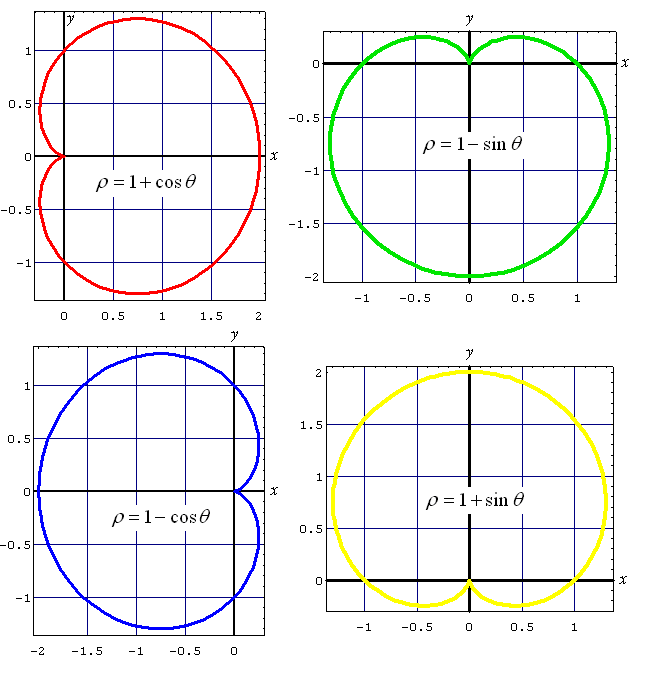
\includegraphics[width=0.5 \linewidth, angle =0]{CardioidsLabeled.png}
  \caption{Cardiod.}
  \label{fig:1}
  \end{figure}
\end{frame}

\begin{frame}
  \textcolor{blue}{Examples}
  Lemniscate:$$ r^2 = 2A^2 cos 2\theta.$$
  \begin{figure}[htbp]
    \centering
    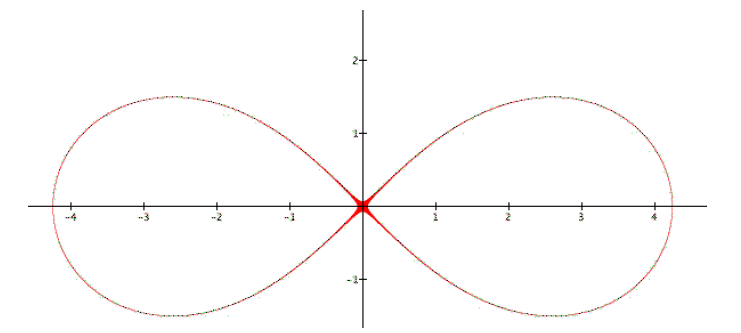
\includegraphics[width=0.8 \linewidth, angle =0]{Lemniscate.png}
    \caption{Lemniscate.}
    \label{fig:2}
    \end{figure}
\end{frame}

\begin{frame}
\textcolor{blue}{Exercise 1}

How to derive this set of formula$(1)(2)(3)$?\\ \pause
~\\
~\\
~\\
~\\
~\\
~\\
\textcolor{blue}{Tips:}\\
If you can derive it by yourself, you can be very confident about kinematics problems in exams.
\end{frame}

\section{Natural Coordinates}
\begin{frame}{Kinematics in 3D: Natural Coordinates}
  \begin{block}{Basic Vectors}
    \begin{enumerate}
      \item $\hat{n_\tau}:$ along the direction of $\vec{v}$
      \item $\hat{n_n}$ and $\hat{n_b}$: perpendicular to the direction of $\vec{v}$
    \end{enumerate}
    $$
      \hat{n_\tau}=\frac{\vec{v}}{|\vec{v}|},\ 
      \hat{n_n}=\frac{\dot{\hat{n_\tau}}}{|\dot{\hat{n_\tau}}|},\ 
      \hat{n_b}=\hat{n_\tau}\times \hat{n_n}
      $$
  \end{block}\pause
  \begin{block}{Basic Formulas}
    $$\vec{v}=v\hat{n_\tau}$$
    $$\vec{a}=\dot{v}\hat{n_\tau}+\frac{v^2}{R_c}\hat{n_n}$$
    $R_c$ means radius of curvature, what is radius of curvature?
  \end{block}
\end{frame}

\begin{frame}
  \textcolor{blue}{Important Tips}
  \begin{enumerate}
    \item Difference between $\dot{\vec{v}}$ and $\dot{v}.$\pause
    \item Difference between \textcolor{red}{normal and tangential}, \textcolor{brown}{radial and transversal} components of velocity and acceleration.
  \end{enumerate}
\end{frame}


\begin{frame}{Kinematics in 3D: Spherical Coordinates (Optional)}
  \begin{block}{Basic Formulas in Spherical Coordinates}
  \begin{align*}
    \vec{r}&= r\hat{n_r}\\
    \vec{v}&= \dot{r}\hat{n_r}+r cos\phi\dot{\theta}\hat{n_\theta}+r\dot{\phi}\hat{n_\phi}\\
    \vec{a}&= (\ddot{r}-r\dot{\theta}^2cos^2 \phi-r\dot{\phi}^2)\hat{n_r}\\ & +(2\dot{r}\dot{\theta}cos\phi-2r\dot{\theta}\dot{\phi}sin\phi+r\ddot{\theta}cos\phi)\hat{n_\theta}\\ & +(2\dot{r}\dot{\phi}+r\dot{\theta}^2cos\phi sin\phi+r\ddot{\phi})\hat{n_\phi}
    \end{align*}
  \end{block}\pause
  How to derive them?
  \textcolor{blue}{\url{http://output.to/sideway/default.aspx?qno=140700003}}
\end{frame}

\begin{frame}
\textcolor{blue}{Exercise 2}\\
\textcolor{blue}{\footnotesize{Cartesian coordinates and natural coordinates}}\\
A particle moves in the $x$-$y$ plane so that$$x(t) = at,\ y(t) = bt^2,$$
where $a, b$ are positive constants. Find its trajectory, velocity, and acceleration (its tangential and
normal components).
\end{frame}

\section{Exercises}
\begin{frame}
  \textcolor{blue}{Exercise 3}\\
  \textcolor{blue}{\footnotesize{Cartesian coordinates and natural coordinates}}\\
  The velocities of two particles observed from a fixed frame of reference are given in the Cartesian
  coordinates by vectors $\vec{v_1}(t) = (0, 2, 0) + (3, 1, 2)t^2$ and $\vec{v_2}(t) = (1, 0, 1).$ At the initial instant of
  time $t = 0$, the positions of these particles are $\vec{r_1}(0) = (1, 0, 0)$ and $\vec{r_2}(0) = (0, 1, 1).$
  \\
  ~\\ \textbf{Find}: the positions of both particles and the acceleration of particle 1 (and its tangential and normal
  components), relative position, and relative acceleration of particle 1 with respect to particle 2 at
  any instant of time $t$.
  \end{frame}

  \begin{frame}
  \textcolor{blue}{Exercise 4}\\
  \textcolor{blue}{\footnotesize{Polar coordinates (Archimedes' spiral)}}\\
  
  A disc of radius $R$ rotates about its axis of symmetry (perpendicular to the disk
surface) with constant angular velocity $\dot{\varphi}=\omega=$ const. At the instant of time $t = 0$ a beetle starts
to walk with constant speed $v_0$ along a radius of the disk, from its center to the edge.\\
\textbf{Find}\\
  (a) the position of the beetle and its trajectory in the Cartesian and polar coordinate systems,\\
  (b) its velocity both systems,\\
  (c) its acceleration in both systems (Cartesian components, polar components, as well as tangential
  and normal components).
\end{frame}

\begin{frame}
\textcolor{blue}{Exercise 5}\\
\textcolor{blue}{\footnotesize{Polar coordinates}}

A particle moves along a hyperbolic spiral (i.e. a curve $r=c/\varphi$, where $c$ is a positive constant), so
that $\varphi(t) = \varphi_0 + \omega t,$ where $\varphi_0$ and $\omega$ are positive constants. \textbf{Find} its velocity and acceleration (all
components and magnitudes of both vectors).
\end{frame}

\begin{frame}
\textcolor{blue}{Exercise 6}

For the situation discussed in \textcolor{blue}{Exercise 3},  answer the following questions.\\
(a) What is the distance covered by the beetle (write down the integral only, do not evaluate it)?\\
(b) What is the radius of curvature of the trajectory?
\end{frame}

\begin{frame}
\textcolor{blue}{Exercise 7}

Four spiders are initially placed at the four corners of a square with side length $a$. The spiders
crawl counter-clockwise at the same speed and each spider crawls directly toward the next spider
at all times. They approach the center of the square along spiral paths.\\ \textbf{Find}\\
(a) polar coordinates of a spider at any instant of time, assuming the origin is at the center of the
square,\\
(b) the time after which all spiders meet,\\
(c) the trajectory of a spider in polar coordinates.
\end{frame}

\begin{frame}
\textcolor{blue}{Exercise 8 (supplement)}

The hall chandelier with a height of $h$ above the ground exploded into fragments, shooting in all directions, the initial velocity was the same as $v_0$, and the fragments would not bounce when them reach the ground. Try to find the radius $R$ of the debris distribution area on the ground.
\begin{figure}[htbp]
\centering
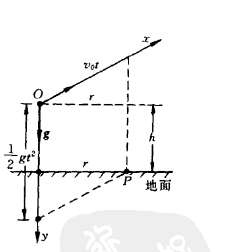
\includegraphics[width=0.4 \linewidth, angle =0]{ex8.png}
%\caption{.}
\label{fig:3}
\end{figure}
\end{frame}

\begin{frame}
\textcolor{blue}{Exercise 9 (supplement)}

Using kinematics method to solve the distribution function $\rho(x)$ of the radius of curvature of the curve $y=e^x$.
\begin{figure}[htbp]
\centering
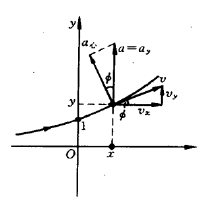
\includegraphics[width=0.45 \linewidth, angle =0]{ex9.png}
%\caption{.}
\label{fig:4}
\end{figure}
\end{frame}

\begin{frame}
\textcolor{blue}{Exercise 10 (supplement)}

The height of the river bank is $h$, and people use ropes to pull the boat to shore. If the angle between the rope and the water surface is $\theta$, the speed of the human left is $v_0$ and the acceleration is $a_0$. Try to find the speed $v$ and acceleration $a$ of the ship at this time.
\begin{figure}[htbp]
\centering
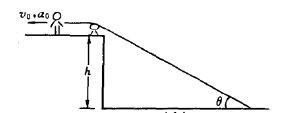
\includegraphics[width=0.5 \linewidth, angle =0]{ex10.png}
%\caption{.}
\label{fig:5}
\end{figure}
\end{frame}

\begin{frame}{Reference}
  \begin{thebibliography}{9}
  \setbeamertemplate{bibliography item}[article]
  \bibitem{C} Yigao Fang.\\
  \textcolor{black}{VP160 Recitation Slides.}\\
  2020
  \bibitem{C} Haoyang Zhang.\\
  \textcolor{black}{VP160 Recitation Slides.}\\
  2020
  \setbeamertemplate{bibliography item}[book]
  \bibitem{C} Yousheng Shu (舒幼生).\\
  \textcolor{black}{\textit{Mechanics (力学)}}\\
  Peking University Press, 2005
  \end{thebibliography}
  \end{frame}

  \end{document}



